\documentclass[a4paper, 12pt]{article}

\usepackage[margin=1in]{geometry}
\usepackage{amsmath}
\usepackage{graphicx}
\usepackage{enumitem}

\title{\Large\textbf{Eigenfaces for Face Recognition}}
\author{Your Name}
\date{\today}

\begin{document}

\maketitle

\section*{Introduction}
This assignment explores the use of Eigenfaces, a Principal Component Analysis (PCA) based approach for face recognition and dimensionality reduction of facial images. We follow the method outlined by Turk and Pentland, where the eigenfaces are derived from the eigenvectors of the covariance matrix of the training set of images.

\section*{Methodology}

\subsection*{The Dataset}
The Olivetti faces dataset was used for this implementation. The dataset consists of face images where:
\begin{itemize}
    \item Each image is 64×64 pixels in grayscale
    \item Each image is flattened into a 4096-dimensional vector
    \item A set of $M$ such images forms a data matrix $X$ of size $M \times N$ (with $N=4096$)
\end{itemize}

\subsection*{Computing the Face Space (Turk and Pentland Method)}
Instead of directly performing an SVD on the large data matrix, the Turk and Pentland method exploits the fact that the number of images $M$ is often much smaller than the dimensionality $N$ of each image. The steps are as follows:

\begin{enumerate}
    \item Compute the mean face:
    \[
    \mu = \frac{1}{M}\sum_{i=1}^{M} x_i
    \]
    where $x_i$ is the $i$-th image as a vector of length $N$.
    
    \item Subtract the mean face from each image to center the dataset:
    \[
    X' = X - \mu
    \]
    Here, $X'$ is still $M \times N$.
    
    \item Construct the covariance matrix in the reduced space:
    \[
    L = X' X'^T \quad \text{(an } M \times M \text{ matrix)}
    \]

    \item Compute the eigenvalues and eigenvectors of $L$:
    \[
    L v_i = \lambda_i v_i
    \]

    \item Since $L$ is $M \times M$, we only obtain $M$ eigenvectors. Each eigenvector $v_i$ in this $M$-dimensional space can be mapped back to the original $N$-dimensional face space:
    \[
    u_i = X'^T v_i
    \]
    The vectors $u_i$ are the eigenfaces.

    \item Normalize each $u_i$ so that it has unit length. The eigenfaces $u_i$ correspond to the directions of maximum variance in the face space.
\end{enumerate}

\subsection*{Dimensionality Reduction}
After computing the eigenfaces, we can reduce the dimensionality:
\begin{itemize}
    \item Select the top $N$ eigenfaces corresponding to the largest eigenvalues.
    \item Project images onto this reduced eigenface subspace:
    \[
    W = U_{N}^T (X' - \mu)
    \]
    where $U_{N}$ is the matrix of top eigenfaces.
    
    \item Each image is now represented by a vector of $N$ dimensions instead of $4096$.
\end{itemize}

In our implementation, we chose $N = 128$.

\subsection*{Image Reconstruction}
To reconstruct an image from its lower-dimensional representation:
\begin{itemize}
    \item Let $w$ be the weight vector corresponding to the projection of an image $x$:
    \[
    w = U_{N}^T(x - \mu)
    \]

    \item Reconstruct the image using:
    \[
    \hat{x} = U_{N} w + \mu
    \]
\end{itemize}

\section*{Results}

\subsection*{Top Eigenfaces}
The following figure shows the top 10 eigenfaces computed from the dataset:

\begin{figure}[h]
    \centering
    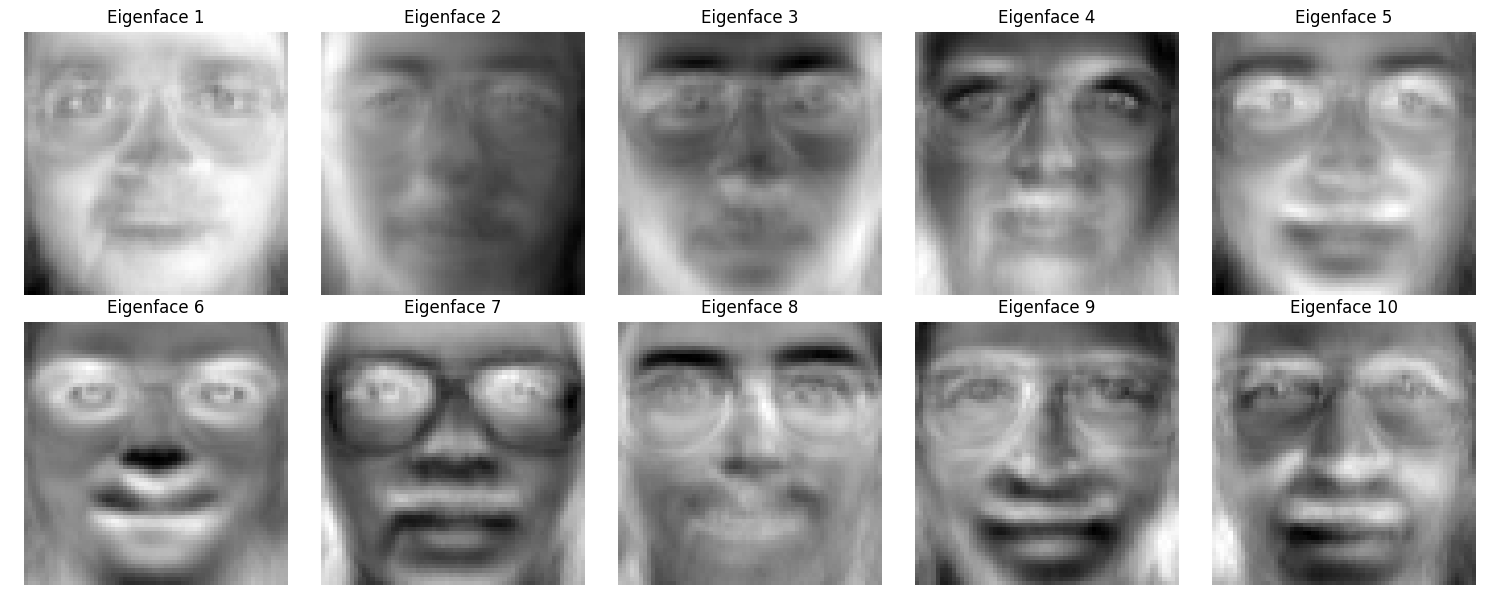
\includegraphics[width=0.8\textwidth]{eigenfaces.png}
    \caption{Top 10 eigenfaces computed from the Olivetti faces dataset}
\end{figure}

\subsection*{Image Reconstruction}
Below is an example of an original image and its reconstruction using 128 eigenface components:

\begin{figure}[h]
    \centering
    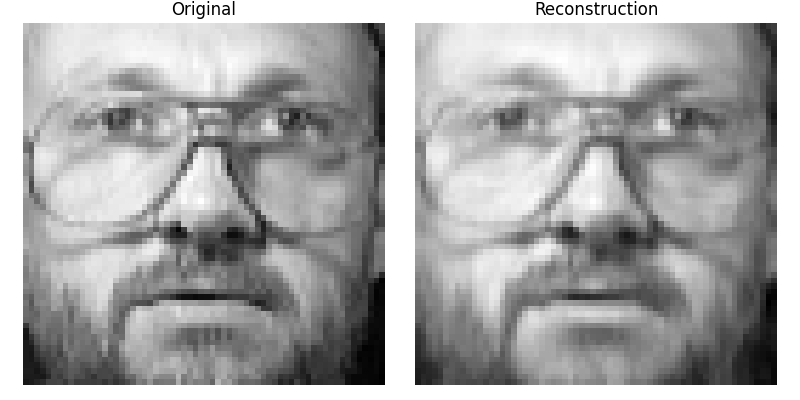
\includegraphics[width=0.8\textwidth]{reconstruction_example.png}
    \caption{Original image (left) and its reconstruction (right)}
\end{figure}

The reconstruction is of good quality while significantly reducing the dimensionality. This demonstrates the effectiveness of the Turk and Pentland eigenface method in capturing the essential features of face images and enabling efficient face recognition and analysis.

\end{document}